\chapter{Schwache Felder, Gravitationswellen und das Wirkungsprinzip}

Die exakten Gleichungen der allgemeinen Relativitätstheorie sind nichtlinear, und ihre Komponentendarstellung kann schon vor der Lösung eines einzigen physikalischen Problems äußerst unübersichtlich werden. Für die letzte Vorlesung des Kurses ist es sinnvoller, das Prinzip von der Rechenarbeit zu trennen. Wir fragen, wie Einsteins Gleichungen im Grenzfall eines schwachen Gravitationsfeldes aussehen, bestimmen die in dieser Näherung enthaltenen Wellen und schließen dann damit, zu sehen, wie sich die vollständigen Feldgleichungen in ein bemerkenswert kompaktes Wirkungsprinzip einfügen.

Drei Fragen strukturieren die Diskussion. Was bedeutet ein schwaches Gravitationsfeld? Warum ist die schwache Theorie linear, die exakte aber nicht? Und welche physikalischen Effekte unterscheiden eine Gravitationswelle von einem bloßen Koordinatenwackeln?

\section{Eine kleine Störung einer Gleichgewichtsgeometrie}

Schwäche ist ein Näherungsverfahren. Ist eine dimensionslose Störung von der Größenordnung \(\epsilon\ll1\), so ist ihr Quadrat von der Größenordnung \(\epsilon^2\), und eine Rechnung erster Ordnung lässt Terme dieser letzteren Ordnung konsequent weg. Ein vertrautes Beispiel ist ein mechanisches System, das kleine Schwingungen um seine Gleichgewichtslage ausführt. Seine exakten Gleichungen können nichtlinear sein, doch hinreichend kleine Schwingungen gehorchen linearen Gleichungen.

In der Gravitation ist die leere flache Raumzeit die Gleichgewichtslösung. Wir beginnen mit Einsteins Vakuumgleichung,
\begin{equation}
 R_{\mu\nu}-\frac12 g_{\mu\nu}R=0.
 \label{eq:l10-vacuum-einstein}
\end{equation}
Ihre Spur in vier Dimensionen zu bilden ergibt
\begin{equation}
 g^{\mu\nu}
 \left(R_{\mu\nu}-\frac12 g_{\mu\nu}R\right)
 =R-2R=-R=0,
\end{equation}
Die Vakuumgleichung ist somit gleichbedeutend mit
\begin{equation}
 R_{\mu\nu}=0.
 \label{eq:l10-ricci-flat}
\end{equation}

\begin{figure}[htbp]
\centering
\includegraphics[width=0.68\textwidth]{lecture_10_figure_02.png}
\caption{Die Vakuumgleichung \(R_{\mu\nu}=0\), die am Anfang der Schwachfeldbetrachtung isoliert wurde.}
\lectureframe{00:03:11}
\end{figure}

Gleichgewicht bedeutet hier eine quellenfreie Lösung ohne Zeitabhängigkeit. Die flache Raumzeit ist die einfachste solche Lösung. Eine Einschränkung ist wesentlich: Flachheit bedeutet nicht, dass die Metrikkomponenten in jedem Koordinatensystem einer bestimmten Matrix entsprechen. Sie bedeutet, dass sich Inertialkoordinaten wählen lassen, in denen
\begin{equation}
 g_{\mu\nu}=\eta_{\mu\nu}.
\end{equation}
Diese Unterscheidung zwischen einer Geometrie und den zu ihrer Beschreibung verwendeten Koordinaten wird bald zum zentralen Knackpunkt.

Stellen wir uns nun eine heftige Quelle vor, etwa ein kompaktes Doppelsternsystem. Ihr Nahfeld kann stark sein, doch weit von der Quelle entfernt breitet sich die Störung aus und wird klein. In einem geeigneten Koordinatensystem lässt sich die Metrik dann schreiben als
\begin{equation}
 g_{\mu\nu}(x)=\eta_{\mu\nu}+h_{\mu\nu}(x),
 \qquad |h_{\mu\nu}|\ll1.
 \label{eq:weak-split}
\end{equation}
Die Störung \(h_{\mu\nu}\) darf von allen vier Raumzeitkoordinaten abhängen. Schwachheit bedeutet, dass Terme höherer als erster Ordnung vernachlässigt werden.

\section{Was in erster Ordnung übrig bleibt}

Der vollständige Ricci-Tensor ist an dieser Stelle zu umfangreich, um nützlich zu sein. Seine Struktur genügt. Christoffel-Symbole enthalten die inverse Metrik und eine Ableitung der Metrik, während die Krümmung eine Ableitung eines Christoffel-Symbols und ein Produkt zweier Christoffel-Symbole enthält:
\begin{equation}
 \Gamma\sim\frac12 g^{-1}\partial g,
 \qquad
 R\sim\partial\Gamma+\Gamma\Gamma.
 \label{eq:curvature-skeleton}
\end{equation}

\begin{figure}[htbp]
\centering
\includegraphics[width=0.84\textwidth]{lecture_10_figure_03.png}
\caption{Die Aufspaltung in schwachen Hintergrund und Störung sowie der schematische Aufbau
\(R\sim\partial\Gamma+\Gamma\Gamma\). Die Schreibweise macht die Ordnungen in
\(h\) sichtbar, ohne alle Indizes auszuschreiben.}
\lectureframe{00:10:17}
\end{figure}

Die inverse Metrik ergibt sich aus
\(g^{\mu\alpha}g_{\alpha\nu}=\delta^\mu{}_\nu\). In erster Ordnung gilt
\begin{equation}
 g^{\mu\nu}=\eta^{\mu\nu}-h^{\mu\nu}+O(h^2),
 \label{eq:inverse-weak}
\end{equation}
wobei die Indizes von \(h\) mit der Hintergrundmetrik angehoben werden. In Inertialkoordinaten ist der Hintergrund konstant,
\begin{equation}
 \partial_\alpha\eta_{\mu\nu}=0,
\end{equation}
und daher
\begin{equation}
 \partial_\alpha g_{\mu\nu}
 =\partial_\alpha h_{\mu\nu}.
\end{equation}
Folglich gilt
\begin{equation}
\begin{aligned}
 \Gamma&=O(\partial h),\\
 R_{\mu\nu}
 &=O(\partial\partial h)+O\bigl((\partial h)^2\bigr)\\
 &\quad+O(h\,\partial\partial h).
\end{aligned}
 \label{eq:ricci-orders}
\end{equation}

\begin{figure}[htbp]
\centering
\includegraphics[width=0.84\textwidth]{lecture_10_figure_04.png}
\caption{Die Entwicklung der inversen Metrik an der Tafel und die Feststellung, dass
\(\partial\eta=0\). In führender Ordnung bleiben nur Ableitungen von \(h_{\mu\nu}\) übrig.}
\lectureframe{00:11:55}
\end{figure}

Die letzten beiden Terme in Gleichung~\eqref{eq:ricci-orders} sind quadratisch in der Störung und werden weggelassen. Die Vakuumgleichungen sind daher lineare Gleichungen mit zweiten Ableitungen von \(h_{\mu\nu}\). Genau das bedeutet Linearisierung. Es ist keine Aussage darüber, dass Einsteins exakte Theorie linear wäre.

\begin{classroomqa}
\audiencequestion{Der Krümmungstensor hat vier Indizes, der Ricci-Tensor dagegen zwei. Wenn zwei Ableitungen bereits Indizes tragen und \(h_{\mu\nu}\) zwei weitere, wie geht die Indexzählung auf?}
\lecturerresponse{Der Ricci-Tensor entsteht durch Kontraktion eines Indexpaares im Krümmungstensor. Die für diese Kontraktion verwendete Metrik lässt zwei freie Indizes übrig, genau das Indexpaar von \(R_{\mu\nu}\). Die symbolische Form \(\partial\partial h\) lässt diese Kontraktionen unausgeschrieben; sie zählt die Ordnungen, ist aber keine vollständige Formel mit ausgeschriebenen Indizes.
\lecturetimestamp{00:18:45--00:19:53}}
\end{classroomqa}

\begin{classroomqa}
\audiencequestion{Führt die Kontraktion mit der inversen Metrik Terme wie \(h\,\partial^2h\) ein, und falls ja, warum darf man sie vernachlässigen?}
\lecturerresponse{Das tut sie. Ersetzt man \(g^{-1}\) durch \(\eta^{-1}-h+\cdots\), erhält man sowohl den linearen Term \(\eta^{-1}\partial^2h\) als auch Korrekturen, die eine zweite Potenz von \(h\) enthalten. Letztere sind quadratisch. Nach derselben Regel werden \(h\,\partial h\), \(h\,\partial^2h\) und \((\partial h)^2\) verworfen. Nur eine Potenz der Störung beizubehalten ist genau die hier vorgenommene Näherung.
\lecturetimestamp{00:19:55--00:21:14}}
\end{classroomqa}

\section{Warum die Gleichungen wie Wellengleichungen aussehen}

Feldgleichungen mit zweiten Ableitungen legen Wellenausbreitung nahe. Für eine skalare Funktion, die sich entlang der \(z\)-Achse bewegt, lautet das Grundbeispiel
\begin{equation}
 \left(\partial_t^2-\partial_z^2\right)\phi=0,
\end{equation}
Zu den Lösungen gehören beliebige nach rechts und links laufende Profile,
\begin{equation}
 \phi(z,t)=f(z-t)+g(z+t).
\end{equation}
In drei Raumdimensionen lautet dieselbe Gleichung
\begin{equation}
 \left(\partial_t^2-\nabla^2\right)\phi=0.
\end{equation}
Aufgrund ihrer Linearität lassen sich Lösungen überlagern: Die Summe zweier Lösungen ist wieder eine Lösung.

Die Gravitation ist kein Skalarfeld. Die Störung hat Tensor-Komponenten, und die Gleichung \(R_{\mu\nu}=0\) scheint zunächst viele Komponentengleichungen zu liefern. Sie sind nicht alle unabhängig; einige sind Zwangsbedingungen, andere spiegeln die Koordinatenfreiheit wider. Die Analogie ist die Maxwell-Theorie: Dort bleibt nach einer Reihe von Feldgleichungen schließlich nur die physikalische transversale Welle übrig.

Nach geeigneter Festlegung der Koordinatenbedingungen erfüllen die strahlenden Komponenten eine gewöhnliche Wellengleichung,
\begin{equation}
 \Box h_{\mu\nu}=0,
 \qquad
 \Box=\eta^{\alpha\beta}\partial_\alpha\partial_\beta.
 \label{eq:linear-wave}
\end{equation}
Die genaue Vorzeichenwahl in \(\Box\) hängt von der Signaturkonvention ab; am Inhalt ändert das nichts. Störungen breiten sich auf dem Lichtkegel aus.

\section{Koordinatenwackeln sind keine Gravitationswellen}

Bevor wir jede Lösung der linearisierten Gleichungen als physikalische Welle akzeptieren, müssen wir auf den Vorbehalt bezüglich der Koordinaten zurückkommen. Der flache Raum lässt sich mit gekrümmten Koordinatenlinien beschreiben. Dann unterscheiden sich seine Metrikkomponenten von ihren kartesischen Werten, obwohl seine Krümmung weiterhin null ist.

Die Tafel selbst liefert das Beispiel. Zeichnen wir gerade kartesische Koordinaten auf ihre flache Oberfläche und schreiben
\begin{equation}
 ds^2=\delta_{mn}\,dx'^m dx'^n.
\end{equation}
Nun versehen wir dieselben Punkte mit leicht gekrümmten Koordinaten,
\begin{equation}
 x'^m=x^m+f^m(x).
 \label{eq:small-coordinate-change}
\end{equation}
Die Differentiale lauten dann
\begin{equation}
 dx'^m=dx^m+\partial_n f^m\,dx^n.
\end{equation}
Setzen wir sie in das Linienelement ein und behalten nur Terme erster Ordnung in \(f\), so erhalten wir
\begin{align}
 ds^2
 &=\delta_{mn}dx^m dx^n\\
 &\quad+\left(\partial_m f_n+\partial_n f_m\right)dx^m dx^n
 +O(f^2).
\end{align}
Eine scheinbare Störung der Form
\begin{equation}
 h_{mn}=\partial_m f_n+\partial_n f_m
 \label{eq:pure-gauge}
\end{equation}
kann also eine Geometrie beschreiben, die sich überhaupt nicht geändert hat. Es ist der flache Raum in leicht gekrümmten Koordinaten.

\begin{figure}[htbp]
\centering
\includegraphics[width=0.84\textwidth]{lecture_10_figure_05.png}
\caption{Die Rechnung zum Koordinatenwackeln an der Tafel. Eine kleine Koordinatenänderung induziert eine scheinbar kleine Größe \(h_{mn}\), obwohl die Tafel flach bleibt.}
\lectureframe{00:27:54}
\end{figure}

Gleichung~\eqref{eq:pure-gauge} ist die linearisierte Form der Koordinaten- oder Eichfreiheit. Um diese Schein-Störungen zu beseitigen, sind zusätzliche Bedingungen erforderlich. Die ausführliche Eichalgebra wird hier nicht entwickelt. Entscheidend ist ihre Rolle: Sie entfernt Änderungen der Beschreibung, bewahrt aber Änderungen der Krümmung. Sind die Koordinatenfreiheit und die Zwangsgleichungen berücksichtigt, reduziert sich der physikalische Inhalt auf zwei unabhängige Wellenpolarisationen.

\begin{figure}[htbp]
\centering
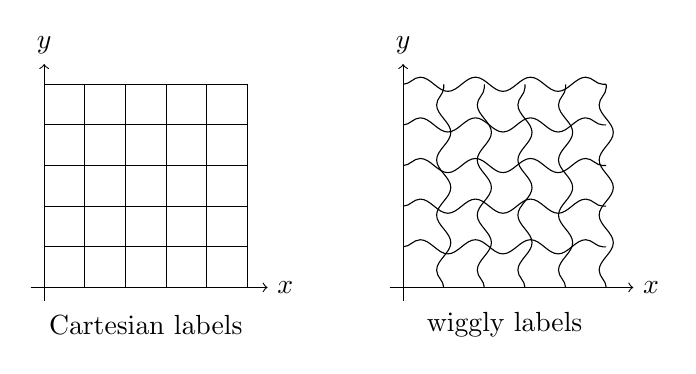
\begin{tikzpicture}[scale=0.86]
\begin{scope}
\draw[->] (-0.2,0) -- (3.3,0) node[right] {$x$};
\draw[->] (0,-0.2) -- (0,3.3) node[above] {$y$};
\foreach \u in {0.6,1.2,1.8,2.4,3.0}{
  \draw (\u,0) -- (\u,3.0);
  \draw (0,\u) -- (3.0,\u);
}
\node at (1.5,-0.55) {Cartesian labels};
\end{scope}
\begin{scope}[xshift=5.3cm]
\draw[->] (-0.2,0) -- (3.4,0) node[right] {$x$};
\draw[->] (0,-0.2) -- (0,3.3) node[above] {$y$};
\foreach \u in {0.6,1.2,1.8,2.4,3.0}{
  \draw[decorate,decoration={snake,amplitude=0.09cm,segment length=0.7cm}]
    (\u,0) -- (\u,3.0);
  \draw[decorate,decoration={snake,amplitude=0.09cm,segment length=0.7cm}]
    (0,\u) -- (3.0,\u);
}
\node at (1.5,-0.55) {wiggly labels};
\end{scope}
\end{tikzpicture}
\caption{Die Geometrie bleibt flach, während sich das Koordinatengitter ändert. Allein anhand der Metrikkomponenten lässt sich nicht entscheiden, ob eine Störung physikalisch ist.}
\end{figure}

\section{Eine Welle, die sich entlang der z-Achse ausbreitet}

Wir wählen eine ebene Welle, die sich in positive \(z\)-Richtung ausbreitet. Ihre Phase lässt sich schreiben als
\begin{equation}
 k(z-t),
\end{equation}
Eine typische Komponente hat dann die Form
\begin{equation}
 h_{\mu\nu}(z,t)
 =h_{\mu\nu}^{(0)}\sin k(z-t).
 \label{eq:plane-wave}
\end{equation}
Flächen konstanter Phase erfüllen \(z-t=\text{constant}\); die Ausbreitungsgeschwindigkeit ist daher gleich der Lichtgeschwindigkeit.

In einer transversalen, spurfrei gewählten Darstellung verschwinden die Komponenten mit einem Zeitindex oder einem \(z\)-Index:
\begin{equation}
 h_{0\mu}=0,
 \qquad
 h_{z\mu}=0.
 \label{eq:tt-transverse}
\end{equation}
Übrig bleibt nur der \(x\)-\(y\)-Block. Er ist symmetrisch und spurfrei:
\begin{equation}
 h_{xy}=h_{yx},
 \qquad
 h_{xx}+h_{yy}=0.
 \label{eq:tt-trace}
\end{equation}

\begin{figure}[htbp]
\centering
\includegraphics[width=0.84\textwidth]{lecture_10_figure_06.png}
\caption{Eine Welle breitet sich entlang \(z\) aus und ist als Folge transversaler Ebenen dargestellt. Die verbleibenden Amplituden im \(x\)-\(y\)-Block erfüllen
\(h_{xx}+h_{yy}=0\).}
\lectureframe{00:43:36}
\end{figure}

Es gibt folglich zwei unabhängige Muster. Für \(i,j\in\{x,y\}\) lassen sie sich darstellen als
\begin{equation}
 h^{\mathrm{TT}}_{ij}(z,t)
 =
 \begin{pmatrix}
 h_+ & h_\times\\
 h_\times & -h_+
 \end{pmatrix}
 \sin k(z-t).
 \label{eq:polarization-matrix}
\end{equation}
Das diagonale Muster heißt Plus-Polarisation. Das nichtdiagonale Muster heißt Kreuz-Polarisation. Eine Drehung der transversalen Achsen um \(45^\circ\) verwandelt das eine Muster in das andere, und eine beliebige linear polarisierte Welle ist eine Überlagerung der beiden. In dieser Theorie gibt es keine weiteren unabhängigen Polarisationen.

\begin{figure}[htbp]
\centering
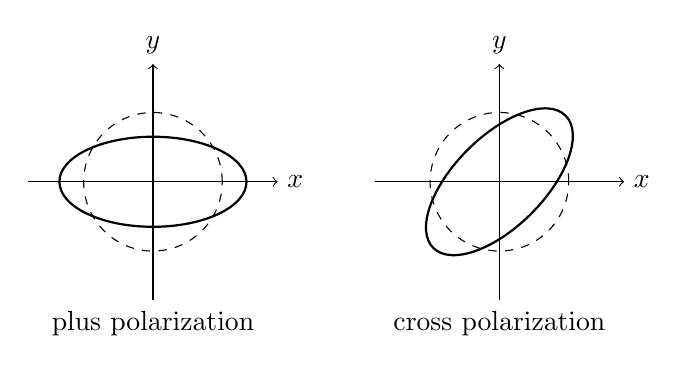
\begin{tikzpicture}[scale=0.88]
\begin{scope}
\draw[->] (-1.8,0) -- (1.8,0) node[right] {$x$};
\draw[->] (0,-1.7) -- (0,1.7) node[above] {$y$};
\draw[dashed] (0,0) circle (1.0);
\draw[thick] (0,0) ellipse (1.35 and 0.65);
\node at (0,-2.05) {plus polarization};
\end{scope}
\begin{scope}[xshift=5.0cm]
\draw[->] (-1.8,0) -- (1.8,0) node[right] {$x$};
\draw[->] (0,-1.7) -- (0,1.7) node[above] {$y$};
\draw[dashed] (0,0) circle (1.0);
\draw[thick,rotate=45] (0,0) ellipse (1.35 and 0.65);
\node at (0,-2.05) {cross polarization};
\end{scope}
\end{tikzpicture}
\caption{Während einer halben Periode wird eine transversale Richtung gedehnt und die dazu senkrechte gestaucht. Eine halbe Periode später kehrt sich die Verformung um.}
\end{figure}

\section{Von den Metrikkomponenten zur physikalischen Dehnung}

Wir halten \(z\) und \(t\) fest und betrachten die transversale Ebene. Für eine reine Plus-Welle gilt
\begin{equation}
 ds_\perp^2
 =(1+h_{xx})\,dx^2+(1-h_{xx})\,dy^2.
 \label{eq:transverse-distance}
\end{equation}
Wenn \(h_{xx}>0\) gilt, ist eine feste Koordinatenstrecke in \(x\)-Richtung geringfügig länger in ihrer Eigenlänge, während die entsprechende Strecke in \(y\)-Richtung geringfügig kürzer ist. Eine halbe Periode später wechselt \(h_{xx}\) sein Vorzeichen, und die Rollen kehren sich um. Ein Quadrat wird abwechselnd horizontal gedehnt und vertikal gestaucht, dann horizontal gestaucht und vertikal gedehnt. Bei der Kreuz-Polarisation findet dieselbe Abwechslung entlang um \(45^\circ\) gedrehter Achsen statt.

Ein zunächst \(L\) langer Arm ändert sich in erster Ordnung um
\begin{equation}
 \frac{\Delta L}{L}\simeq\frac12 h_{ij}n^i n^j,
 \label{eq:fractional-strain}
\end{equation}
wobei \(\mathbf n\) in Richtung des Arms zeigt. Diese Formel übersetzt die Metrikstörung in die dimensionslose Dehnung, die ein Detektor misst.

\begin{classroomqa}
\audiencequestion{Ein Meterstab wird elektromagnetisch zusammengehalten und ändert seine Ruhelänge nicht einfach mit den Koordinaten. Sollte man in der Darstellung stattdessen frei aufgehängte Testmassen verwenden?}
\lecturerresponse{Diese Unterscheidung ist wichtig. Ein realer Stab hat elastische Eigenschaften, daher erzeugt das Gezeitenfeld Spannungen in seinem Inneren; ein Stahlstab und ein Holzstab reagieren im Allgemeinen unterschiedlich stark. Frei aufgehängte Testmassen vermeiden diese spezielle elastische Reaktion und machen die Relativbeschleunigung unmittelbarer sichtbar. In beiden Fällen benennt die vorbeiziehende Welle die Punkte nicht bloß um. Ihre zeitabhängige Krümmung hat eine physikalische Wirkung.
\lecturetimestamp{00:47:23--00:48:48}}
\end{classroomqa}

Die genaue lokale Aussage ist die geodätische Abweichung. Für benachbarte frei fallende Teilchen mit dem Abstand \(\xi^i\) gilt
\begin{equation}
 \frac{d^2\xi^i}{dt^2}
 =-R^i{}_{0j0}\,\xi^j.
 \label{eq:geodesic-deviation}
\end{equation}
In der schwachen transversalen, spurfrei gewählten Welle gilt
\begin{equation}
 R_{0i0j}=-\frac12\ddot h^{\mathrm{TT}}_{ij},
 \label{eq:tidal-curvature}
\end{equation}
Die oszillierende Metrik erzeugt somit eine wechselnde Gezeitenbeschleunigung. Deshalb lässt sich eine zeitabhängige Welle nicht als statische Wahl von Maßstäben abtun. Sie hat eine von null verschiedene Krümmung.

\begin{classroomqa}
\audiencequestion{Was kann Dehnung und Stauchung messen, wenn alle Maßstäbe in der Umgebung beeinflusst werden?}
\lecturerresponse{Ein Dehnungsmessstreifen kann die reale Spannung erfassen, die in einem Materialkörper entsteht. Noch besser lässt sich der veränderliche Abstand frei aufgehängter Massen überwachen. Eine statische, gleichförmige Skalierung könnte in den Messapparat aufgenommen werden, doch die oszillierende Krümmung bewirkt eine Reaktion, die sich aufzeichnen lässt.
\lecturetimestamp{00:51:10--00:52:02}}
\end{classroomqa}

\section{Quellen und Detektoren}

Elektromagnetische Wellen entstehen durch bewegte Ladungen und Ströme. Gravitationswellen entstehen durch bewegte Massen- und Energieverteilungen. Die Erhaltung von Energie und Impuls schließt Gravitations-Monopol- und -Dipolstrahlung für ein isoliertes System aus, sodass das führende strahlende Moment quadrupolar ist. Ein kompaktes Doppelsternsystem liefert genau das erforderliche zeitlich veränderliche Quadrupolmoment: Zwei dichte Körper umkreisen einander und senden Wellen in das Fernfeld aus.

In der Nähe des Doppelsternsystems ist die Raumzeit stark gekrümmt, und die lineare Entwicklung in Gleichung~\eqref{eq:weak-split} ist unzuverlässig. In großer Entfernung breitet sich die auslaufende Welle über eine größere Fläche aus, ihre Amplitude wird klein und die linearisierte Beschreibung wird genau. Für einen Beobachter auf der \(z\)-Achse der Quelle liegen die messbaren Dehnungen in der transversalen \(x\)-\(y\)-Ebene.

\begin{classroomqa}
\audiencequestion{Ist der Maßstab in der Zeichnung ein abstrakter Koordinatenmaßstab oder ein physischer Meterstab, und wie könnte ein veränderlicher Maßstab den Effekt messen?}
\lecturerresponse{Es kann sich um einen physischen Gegenstand handeln, doch dann spielen seine Materialeigenschaften eine Rolle. Die Krümmung erzeugt die Gezeitenspannung; Stahl und Holz müssen sich darunter nicht gleich verformen. Schon der Vergleich ihrer Reaktionen ist eine Messung. Ein sauberer arbeitender Detektor ersetzt die Stäbe durch getrennte Testmassen und misst ihre Relativbewegung.
\lecturetimestamp{00:54:00--00:55:19}}
\end{classroomqa}

Ein Resonanzdetektor ist eine mögliche Strategie. Hat ein mechanisches System eine Eigenfrequenz nahe der Frequenz der einlaufenden Welle, treibt die Welle das System kohärent an und verstärkt die Reaktion. Ein Interferometer nutzt eine andere Strategie: Spiegel dienen als Testmassen, und Laserinterferenz vergleicht die effektiven Längen senkrechter Arme. Eine Plus-polarisierte Welle verlängert den einen Arm und verkürzt den anderen – genau das differentielle Signal, für dessen Nachweis ein Interferometer ausgelegt ist.

\begin{classroomqa}
\audiencequestion{Wäre das die Grundlage eines Gravitationswellendetektors?}
\lecturerresponse{Ja. Ein steifer Stab ändert seine Länge kaum, wohingegen frei aufgehängte Endmassen eine Relativbeschleunigung erfahren können. Man kann auch Resonanz nutzen, sodass ein schwacher periodischer Antrieb eine größere Reaktion hervorruft. Die erwartete astrophysikalische Dehnung ist außerordentlich klein, von der Größenordnung \(10^{-21}\). Die Kunst des Detektorentwurfs besteht darin, diese winzige Relativbewegung in ein messbares Signal umzuwandeln.
\lecturetimestamp{00:55:20--00:57:10}}
\end{classroomqa}

\begin{classroomqa}
\audiencequestion{Ist LIGO ein Beispiel für einen solchen Detektor?}
\lecturerresponse{Ja. Seine grundlegenden Messgrößen ergeben sich aus Laserlicht, das zwischen Spiegeln in senkrechten Armen reflektiert wird. Eine Gravitationswelle verändert die relativen optischen Weglängen und damit das Interferenzmuster. Zum Zeitpunkt dieser Vorlesung hatte das Instrument noch keine direkte Detektion erzielt; das änderte sich später.\editorialnote{Die erste direkte Beobachtung, GW150914, wurde 2015 aufgezeichnet und 2016 bekannt gegeben.}
\lecturetimestamp{00:57:16--00:58:05}}
\end{classroomqa}

\begin{classroomqa}
\audiencequestion{Welche Ausbreitungsgeschwindigkeit folgt aus der Wellenlösung?}
\lecturerresponse{Die Lichtgeschwindigkeit. Die Phase \(k(z-t)\) legt in \(z\) eine Einheit zurück, während \(t\) um eine Einheit zunimmt, und die linearisierte Einstein-Gleichung hat dieselbe Ausbreitungsstruktur entlang des Lichtkegels wie die elektromagnetische Wellengleichung.
\lecturetimestamp{00:58:07--00:58:16}}
\end{classroomqa}

Kollisionen schwarzer Löcher und kompakte Doppelsternsysteme sind besonders vielversprechende Quellen. In der Nähe der Kollision ist das Gravitationsfeld heftig nichtlinear, und ein erheblicher Teil der freigesetzten Energie kann als Gravitationsstrahlung entweichen. Wenn das Signal einen weit entfernten Detektor erreicht, ist seine Amplitude so schwach, dass die lineare Wellenausbreitung eine ausgezeichnete Beschreibung liefert. Gravitationsstrahlung eröffnet damit einen astronomischen Beobachtungskanal, der nicht auf ausgesandtes Licht angewiesen sein muss.

\section{Der Binärpulsar und indirekte Nachweise}

Strahlung transportiert Energie. Sendet ein Doppelsternsystem Gravitationswellen aus, nimmt seine Bahnenergie ab, die Körper nähern sich langsam spiralförmig an, und die Umlaufperiode ändert sich. Der Binärpulsar liefert eine so präzise Uhr, dass sich diese Änderung messen lässt. Seine beobachtete Bahnentwicklung stimmt quantitativ mit dem Energieverlust überein, den die allgemeine Relativitätstheorie vorhersagt.

Im historischen Kontext der Vorlesung war dies der entscheidende indirekte Nachweis: Noch hatte kein Detektor eine durch die Erde laufende Welle registriert, doch der Umlauf verlor Energie genau in der von der Gravitationsstrahlung geforderten Rate. Die Wellen waren bereits durch ihre Wirkung auf ihre Quelle beobachtbar.

\begin{classroomqa}
\audiencequestion{Welche Frequenz oder Periode kennzeichnet das ursprüngliche Binärpulsar-System? Liegt sie im Millisekundenbereich?}
\lecturerresponse{Der Millisekundenbereich bezieht sich auf die Rotation eines Pulsars, nicht auf den Umlauf der beiden Sterne. Im Hörsaal wird der Wert überprüft; die Umlaufperiode beträgt etwa \(7.75\) Stunden. Diese Unterscheidung ist wichtig: Die Gravitationsstrahlung hängt mit der Bahnbewegung des Doppelsternsystems zusammen, während die Radiopulse die präzise Uhr liefern, mit der sie verfolgt wird.
\lecturetimestamp{01:01:27--01:03:28}}
\end{classroomqa}

\begin{classroomqa}
\audiencequestion{Wie stark änderte sich die aufsummierte Umlaufzeitmessung während der Jahrzehnte der Beobachtung?}
\lecturerresponse{Die angegebene aufsummierte Verschiebung beträgt ungefähr dreißig Sekunden. Die momentane relative Änderung ist winzig, doch jahrzehntelange präzise Messungen der Pulsankunftszeiten machen den kumulierten Effekt sichtbar.
\lecturetimestamp{01:03:34--01:03:54}}
\end{classroomqa}

\section{Zeitabhängigkeit, Krümmung und die Grenzen der Linearität}

\begin{classroomqa}
\audiencequestion{Warum wählt man die transversale \(x\)-\(y\)-Ebene? Was ergibt sich, wenn man stattdessen eine Ebene betrachtet, die \(x\) und \(t\) umfasst?}
\lecturerresponse{Die Welle selbst hängt sowohl von \(z\) als auch von \(t\) ab, doch transversal bezeichnet die räumlichen Richtungen senkrecht zu ihrer räumlichen Ausbreitungsrichtung. Bei einer Welle, die sich entlang \(z\) ausbreitet, lassen sich die physikalischen Metrikamplituden im \(x\)-\(y\)-Block wählen. Andere scheinbare Komponenten fehlen oder lassen sich als Koordinatenwackeln entfernen.
\lecturetimestamp{01:02:22--01:03:17}}
\end{classroomqa}

\begin{classroomqa}
\audiencequestion{Oszilliert die Zeit selbst?}
\lecturerresponse{Nein. Die Welle oszilliert als Funktion der Zeit. An einem festen räumlichen Ort ändern sich die Komponenten \(h_{ij}(z,t)\) periodisch. Die Zeit ist eine Koordinate, von der das Feld abhängt, und in dieser Darstellung kein Objekt, das abwechselnd gedehnt und gestaucht wird.
\lecturetimestamp{01:04:00--01:04:18}}
\end{classroomqa}

\begin{classroomqa}
\audiencequestion{Wenn alle \(h_{0\mu}\) verschwinden, gibt es dann keine Krümmung mit Bezug zur Zeitrichtung?}
\lecturerresponse{Doch. Die verbleibenden räumlichen Komponenten hängen von der Zeit ab, und die Krümmung enthält ihre zweiten Ableitungen. Daher erzeugen Ableitungen wie \(\partial_t^2h_{ij}\) Komponenten \(R_{0i0j}\). Dass die Komponenten mit Zeitindex von \(h_{\mu\nu}\) verschwinden, bedeutet nicht, dass auch die zeitabhängige Krümmung verschwindet.
\lecturetimestamp{01:05:15--01:06:09}}
\end{classroomqa}

Die lineare Wellengleichung ergab sich daraus, dass \(h\) als klein angenommen wurde, und nicht daraus, dass Koordinatenartefakte entfernt wurden. Das sind zwei getrennte Schritte. Die Eichfixierung identifiziert die physikalischen Freiheitsgrade; die Linearisierung verwirft nichtlineare Wechselwirkungen.

\begin{classroomqa}
\audiencequestion{Einsteins Gleichungen sind nichtlinear, doch die resultierende Wellengleichung ist linear. Entsteht diese Linearität dadurch, dass unphysikalische Lösungen entfernt werden?}
\lecturerresponse{Nein. Sie entsteht durch die Näherung kleiner Amplituden. Terme mit zwei Potenzen von \(h\) wurden verworfen. Das Entfernen von Koordinatenwackeln entscheidet, welche Lösungen physikalisch sind; dadurch wird die Gleichung nicht linear.
\lecturetimestamp{01:06:45--01:07:29}}
\end{classroomqa}

\begin{classroomqa}
\audiencequestion{Wie groß ist der Fehler gegenüber einer exakten Lösung, nachdem man die linearisierte Gleichung gelöst hat?}
\lecturerresponse{Die ersten weggelassenen Korrekturen sind von der Ordnung \(h^2\). Wenn \(h\sim10^{-1}\), sind sie von der Ordnung \(10^{-2}\); wenn \(h\sim10^{-3}\), sind sie von der Ordnung \(10^{-6}\). Bei einer Störungsrechnung muss man anschließend stets prüfen, ob der angenommene kleine Parameter tatsächlich klein war.
\lecturetimestamp{01:07:35--01:08:31}}
\end{classroomqa}

\begin{classroomqa}
\audiencequestion{Verliert die Welle ihren transversalen Charakter, wenn Terme höherer Ordnung wichtig werden?}
\lecturerresponse{Der wesentliche transversale Charakter der Strahlung bleibt erhalten, nicht aber die lineare Superposition. Starke Wellen wechselwirken mit dem Gravitationsfeld, das andere Wellen tragen; statt unverändert aneinander vorbeizulaufen, werden sie gestreut.
\lecturetimestamp{01:08:34--01:09:11}}
\end{classroomqa}

\begin{classroomqa}
\audiencequestion{Die Ausbreitungsgeschwindigkeit einer mechanischen Welle hängt von Steifigkeit und Dichte ab. Gibt es einen vergleichbaren Sinn, in dem die Raumzeit eine Steifigkeit besitzt?}
\lecturerresponse{Nur im übertragenen Sinn. Bei einem materiellen Medium hängt die Ausbreitung von einer Kombination wie Steifigkeit geteilt durch Dichte ab. Da sich elektromagnetische und Gravitationswellen mit \(c\) ausbreiten, würde man das Medium in der älteren mechanischen Ausdrucksweise als außerordentlich steif bezeichnen. Die moderne Physik schreibt der Raumzeit keinen gewöhnlichen Elastizitätsmodul zu; die invariante Tatsache ist die durch die Feldgleichungen festgelegte Ausbreitung mit Lichtgeschwindigkeit.
\lecturetimestamp{01:09:12--01:11:10}}
\end{classroomqa}

\section{Ein zweiter Zugang: stationäre Wirkung}

Nach der Diskussion der Wellen bleibt Zeit für einen letzten Perspektivwechsel. Das Prinzip der stationären Wirkung bildet die gemeinsame Sprache der klassischen Mechanik, des Elektromagnetismus, der Feldtheorie und des Standardmodells. Die allgemeine Relativitätstheorie gehört zu derselben Struktur.

Für ein Teilchen ist die Wirkung ein Integral entlang einer Bahn. Bei einem Feld ordnet eine Geschichte jedem Punkt der Raumzeit einen Feldwert \(\phi(x)\) zu, und die Wirkung ist ein Integral über die Raumzeit:
\begin{equation}
 S[\phi]
 =\int d^4x\,
 \mathcal L\bigl(\phi,\partial_\mu\phi\bigr).
 \label{eq:field-action}
\end{equation}
Jedes hinreichend reguläre \(\phi(x)\) ist eine denkbare Geschichte, so wie jeder hinreichend reguläre Weg eine denkbare Teilchenbahn ist; die meisten davon sind jedoch keine Lösungen. Die physikalischen Geschichten sind stationäre Punkte der Wirkung bei festgehaltenen Randdaten:
\begin{equation}
 \delta S=0.
 \label{eq:stationary-action}
\end{equation}
Bei einem Feld umschließt der Rand ein Raumzeitgebiet, statt lediglich die beiden Endpunkte eines Weges festzulegen. Die Euler--Lagrange-Gleichungen bestimmen dann die Interpolation zwischen den vorgegebenen Randwerten.

Einsteins Feldgleichungen lassen sich genau auf diese Weise herleiten. Die Variation ist lang, doch die Wirkung selbst ist einfach. Bevor wir sie hinschreiben, brauchen wir das richtige Maß für das Raumzeitvolumen.

\section{Warum die Determinante das Volumen misst}

Wir beginnen in zwei Dimensionen mit einer Diagonalmetrik,
\begin{equation}
 ds^2=g_{xx}\,dx^2+g_{yy}\,dy^2.
\end{equation}
Ein Koordinatenrechteck mit Seitenlängen \(dx\) und \(dy\) hat Eigenlängen \(\sqrt{g_{xx}}\,dx\) und \(\sqrt{g_{yy}}\,dy\); seine Eigenfläche beträgt daher
\begin{equation}
 dA
 =\sqrt{g_{xx}g_{yy}}\,dx\,dy.
\end{equation}
Ist die außerdiagonale Komponente \(g_{xy}\) vorhanden, müssen die Koordinatenkanten nicht senkrecht aufeinander stehen. Die korrigierte Fläche lautet
\begin{equation}
 dA
 =\sqrt{g_{xx}g_{yy}-g_{xy}^2}\,dx\,dy
 =\sqrt{\det g}\,dx\,dy.
 \label{eq:area-determinant}
\end{equation}

\begin{figure}[htbp]
\centering
\includegraphics[width=0.84\textwidth]{lecture_10_figure_07.png}
\caption{Die Verallgemeinerung an der Tafel: vom kleinen Koordinatenrechteck zum Eigenflächenelement \(\sqrt{\lvert g\rvert}\,dx\,dy\). Die Determinante berücksichtigt sowohl die Diagonallängen als auch die außerdiagonale Scherung.}
\lectureframe{01:21:25}
\end{figure}

Dieselbe Konstruktion funktioniert in beliebiger Dimension:
\begin{equation}
 dV_n=\sqrt{|\det g|}\,d^nx.
\end{equation}
Für eine Lorentzsche Raumzeit mit \(g=\det(g_{\mu\nu})\) schreibt man das invariante Vier-Volumenelement üblicherweise als
\begin{equation}
 dV_4=\sqrt{|g|}\,d^4x,
 \label{eq:four-volume}
\end{equation}
oder als \(\sqrt{-g}\,d^4x\) in der Konvention mit überwiegend positiver Signatur. Die Koordinaten eines Gebiets können sich ändern, sein physikalisches Vier-Volumen bleibt jedoch unverändert.

Multipliziert man dieses Maß mit einem beliebigen Skalar \(F(x)\) und integriert, erhält man eine koordinateninvariante Größe:
\begin{equation}
 \int d^4x\,\sqrt{|g|}\,F(x).
 \label{eq:invariant-scalar-integral}
\end{equation}
Die Wirkung einer allgemein kovarianten Theorie sollte diese Form haben. Andernfalls könnten die daraus hergeleiteten Feldgleichungen von einer beliebigen Koordinatenwahl abhängen.

\section{Die Einstein--Hilbert-Wirkung}

Bei reiner Gravitation ist das dynamische Feld die Metrik selbst. Der einfachste nichtkonstante Skalar, der sich aus der Metrik und ihren ersten beiden Ableitungen bildet, ist der Skalar \(R\). Auch eine Konstante ist ein Skalar; ihr Koeffizient ist die kosmologische Konstante. Bis auf Vorzeichenkonventionen und Randterme lautet eine übliche Normierung der Gravitationswirkung
\begin{equation}
 S_{\mathrm{grav}}
 =
 \frac{1}{16\pi G}
 \int d^4x\,\sqrt{|g|}\,(R-2\Lambda).
 \label{eq:einstein-hilbert}
\end{equation}

\begin{figure}[htbp]
\centering
\includegraphics[width=0.84\textwidth]{lecture_10_figure_08.png}
\caption{Das Bild der Feldgeschichte und die Gravitationswirkung an der Tafel. Die skalare Krümmung liefert die Dynamik; der konstante Term ist proportional zum Raumzeitvolumen.}
\lectureframe{01:26:32}
\end{figure}

Der zu \(\Lambda\) proportionale Term ist schlicht ein Vielfaches des gesamten Raumzeitvolumens. Die zuvor entwickelte Wellengleichung galt für das Vakuum mit \(\Lambda=0\), daher trat dieser Term dort nicht auf.

Materie wird durch eine Materiewirkung ergänzt,
\begin{equation}
 S=S_{\mathrm{grav}}+S_{\mathrm{matter}}.
\end{equation}
Im Elektromagnetismus etwa wird der invariante Feldbeitrag aus dem antisymmetrischen Tensor \(F_{\mu\nu}\) gebildet:
\begin{equation}
 S_{\mathrm{EM}}
 =-\frac14
 \int d^4x\,\sqrt{|g|}\,
 F_{\mu\nu}F^{\mu\nu}.
\end{equation}
Die Variation der Gesamtwirkung nach der inversen Metrik definiert den Energie-Impuls-Tensor und ergibt
\begin{equation}
 R_{\mu\nu}
 -\frac12 g_{\mu\nu}R
 +\Lambda g_{\mu\nu}
 =8\pi G\,T_{\mu\nu}.
 \label{eq:einstein-from-action}
\end{equation}
Die kompakte Wirkung enthält somit die vollständigen Feldgleichungen. Im Vakuum und für \(\Lambda=0\) geht sie in die Theorie über, die den zuvor untersuchten Gravitationswellen zugrunde lag.

\begin{classroomqa}
\audiencequestion{Wo geht der Energie-Impuls-Tensor in das Wirkungsprinzip ein?}
\lecturerresponse{Er stammt aus den zusätzlichen Termen, die Materie und andere Felder beschreiben. Elektromagnetische Energie, Teilchenfelder und alle anderen materiellen Inhalte tragen zu \(S_{\mathrm{matter}}\) bei. Die Variation nach der Metrik liefert \(T_{\mu\nu}\). Das Integral, dessen Integrand nur \(\sqrt{|g|}R\) enthält, beschreibt die Vakuum-Gravitationstheorie.
\lecturetimestamp{01:27:26--01:28:25}}
\end{classroomqa}

Die Herleitung ist konzeptionell unkompliziert, algebraisch aber mühsam. Man bildet aus der Metrik die Christoffelsymbole, konstruiert daraus die Krümmung, kontrahiert sie zu \(R\), multipliziert mit dem Determinantenfaktor und variiert den entstehenden Ausdruck. In der Vorlesung scherzt der Dozent, die Rechnung sollte fünf Minuten dauern und wer daran scheitere, falle durch den Kurs. Gleich darauf räumt er ein, dass er die Rechnung nach wesentlich längeren Versuchen schon viele Male aufgegeben hat. Der Scherz bringt einen ernsten Punkt zum Ausdruck: Kompakte Prinzipien müssen keine kurzen Komponentenrechnungen bedeuten.

\begin{classroomqa}
\audiencequestion{Wird die vollständige Variation in einem Relativitätstheorie-Lehrbuch normalerweise ausgeschrieben?}
\lecturerresponse{Das ist möglich, füllt aber viele Seiten. Eine lange Rechnung wird erst dann aufschlussreich, wenn man genügend weit selbst durch sie hindurchgeht, um zu verstehen, warum der nächste Schritt folgt; passives Lesen von Zeile zu Zeile führt selten zu diesem Verständnis. Moderne symbolische und numerische Werkzeuge können einen großen Teil der Rechenarbeit übernehmen, ersetzen aber nicht das leitende Prinzip.
\lecturetimestamp{01:31:10--01:34:16}}
\end{classroomqa}

Für solche Rechnungen gibt es traditionell zwei Wege. Entweder entwickelt man eine so starke geometrische Intuition, dass man erkennt, welche Kombinationen von Tensoren möglich sind, oder man führt die Algebra sorgfältig aus. Meist wird beides miteinander verbunden, häufig mit einem Computer für die längsten Kontraktionen. Der Kurs hat bewusst die Prinzipien betont, die unabhängig davon gelten, welchen Weg man einschlägt.

\begin{classroomqa}
\audiencequestion{Im Rückblick wirkt das Wirkungsprinzip sehr naheliegend. Warum dauerte es von der speziellen bis zur allgemeinen Relativitätstheorie so viele Jahre, und arbeitete Einstein von Anfang an auf die endgültige Theorie hin?}
\lecturerresponse{Der Endpunkt erscheint einfacher, sobald die nötige Geometrie bekannt ist. Damals war die erforderliche Differentialgeometrie den meisten Physikern fremd, und Einstein musste sie mit mathematischer Unterstützung erlernen und weiterentwickeln, insbesondere mit der Hilfe von Marcel Grossmann. Die Begriffe der gekrümmten Raumzeit aufzubauen und in etwa einem Jahrzehnt die richtige Feldgleichung zu finden, war keine langsame Leistung. Die frühen und die abschließenden Arbeiten sind gerade deshalb lesenswert, weil sie zeigen, wie viel unterwegs erst entwickelt werden musste.
\lecturetimestamp{01:34:20--01:35:59}}
\end{classroomqa}

Das Quartal endet somit mit zwei einander ergänzenden Darstellungen derselben Theorie. Die Feldgleichung beschreibt, wie die Krümmung lokal auf den Energie-Impuls reagiert. Das Wirkungsprinzip besagt, dass die gesamte Raumzeitgeschichte ein stationärer Punkt eines invarianten Funktionals ist. Im schwachen Fernfeld gehen beide Beschreibungen in transversale Wellen über, die reale Krümmung mit Lichtgeschwindigkeit transportieren.